\documentclass[man,apacite,draftfirst]{apa6} \usepackage{amsmath}
\usepackage{float} \usepackage{graphicx} \usepackage{mathrsfs}

\title{Detection of Feedback Contingency Depends on Declarative Systems}
\shorttitle{Declarative Feedback Contingency}

\threeauthors {Matthew J. Crossley} {W. Todd Maddox} {F. Gregory Ashby}
\threeaffiliations {SRI International} {University of California, Santa Barbara}
{University of Texas at Austin}

\abstract{Individuals in drug rehabilitation often experience relapse when
returned to the original context of their drug use. Why do treatments generalize
so poorly across different contexts? We recently addressed this question in the
domain of procedural learning, which is thought to play an important role in
forms of addiction, bad habits, and other maladaptive states
\cite{crossley_erasing_2013}. Our work suggests that feedback contingency,
defined as the correlation between response confidence and outcome, plays a
vital role in controlling a gate that normally prevents procedural knowledge
from being modified during interventions. In particular, our results suggested
that modification of procedural knowledge is possible only if feedback
contingency is high. Here, we ask whether the estimation of feedback contingency
depends on declarative mechanisms (e.g., prefrontal networks involved in working
memory and executive reasoning). Our rationale is as follows: If feedback
contingency is computed by declarative mechanisms, then increasing cognitive
load during intervention via the concurrent performance of an additional task
should disrupt the accurate estimation of contingency, thereby keeping the gate
on procedural learning open. We report the results from an experiment following
this logic that suggests that feedback contingency estimation is indeed
supported by declarative systems.}

\rightheader{Dual-Task Unlearning} \leftheader{Dual-Task Unlearning}

\begin{document}
\maketitle

\section*{Introduction}
Relapse often occurs when an addict returns to the original context of their
drug use \cite{higgins_outpatient_1995}. This may occur because interventions
given in clinics do not modify addiction-driving stimulus-response (SR)
associations, but rather entail the learning of new clinic-specific
associations. Returning to the original context of drug abuse then reactivates
the preserved addiction-driving SR associations, causing relapse. If true, then
this hypothesis means that the brain has a gating mechanism to protect learning
obtained in old contexts from being modified. Our prior work, which was focused
on understanding this gating mechanism \cite{crossley_erasing_2013}, found that
feedback contingency -- defined as the correlation between response confidence
and outcome -- was a principle driver of this gate. The present study is an
extension of this earlier work, asking whether the estimation of feedback
contingency depends on declarative mechanisms. The rest of the introduction
proceeds with a brief summary of the key findings reported by
\cite{crossley_erasing_2013}, followed by the logic of the current study.

\subsection*{Crossley et al. (2013)}
\cite{crossley_erasing_2013} attempted to understand why the SR associations
underlying procedural learning, habits, and addiction are so remarkably
resistant to modification \cite{crossley_erasing_2013}. We developed a task
that, after initial acquisition of SR associations, attempted to erase the
just-formed engram. The results showed promising initial signs of true memory
erasure.

Our experiments included three phases of equal duration: acquisition,
intervention, and test. During acquisition, all participants were trained on the
II categories shown in panel C of Figure \ref{fig:test_cats}. During
intervention, the category structure was unchanged, but feedback indicating the
correctness of responses was manipulated in an attempt to erase the learning
that occurred during the initial acquisition. The core idea was to erase
initially acquired SR associations by overwriting them with random feedback
(RF). In the RF(.25) conditions, the feedback suddenly became random and since
there are four categories, each subject was given positive feedback with
probability .25 on every trial and negative feedback with probability .75. In
the mixed feedback conditions, RF was given with probability .75 and true
feedback was given with probability .25. Finally, in the RF(.40) conditions, RF
was also given, but the probability of positive feedback was .40. Next, during
test, feedback was returned to 100\% veridical. Half the subjects in each
condition relearned the original categories (the relearning conditions) and half
learned new categories that used the same stimuli but permuted the
category-response mappings. Thus the study included six conditions created from
a 3 $\times$ 2 factorial design where three levels of intervention feedback
[RF(.25), RF(.40), mixed feedback] were crossed with two levels of test
(relearning, new learning).

\begin{figure}[t]
\centering 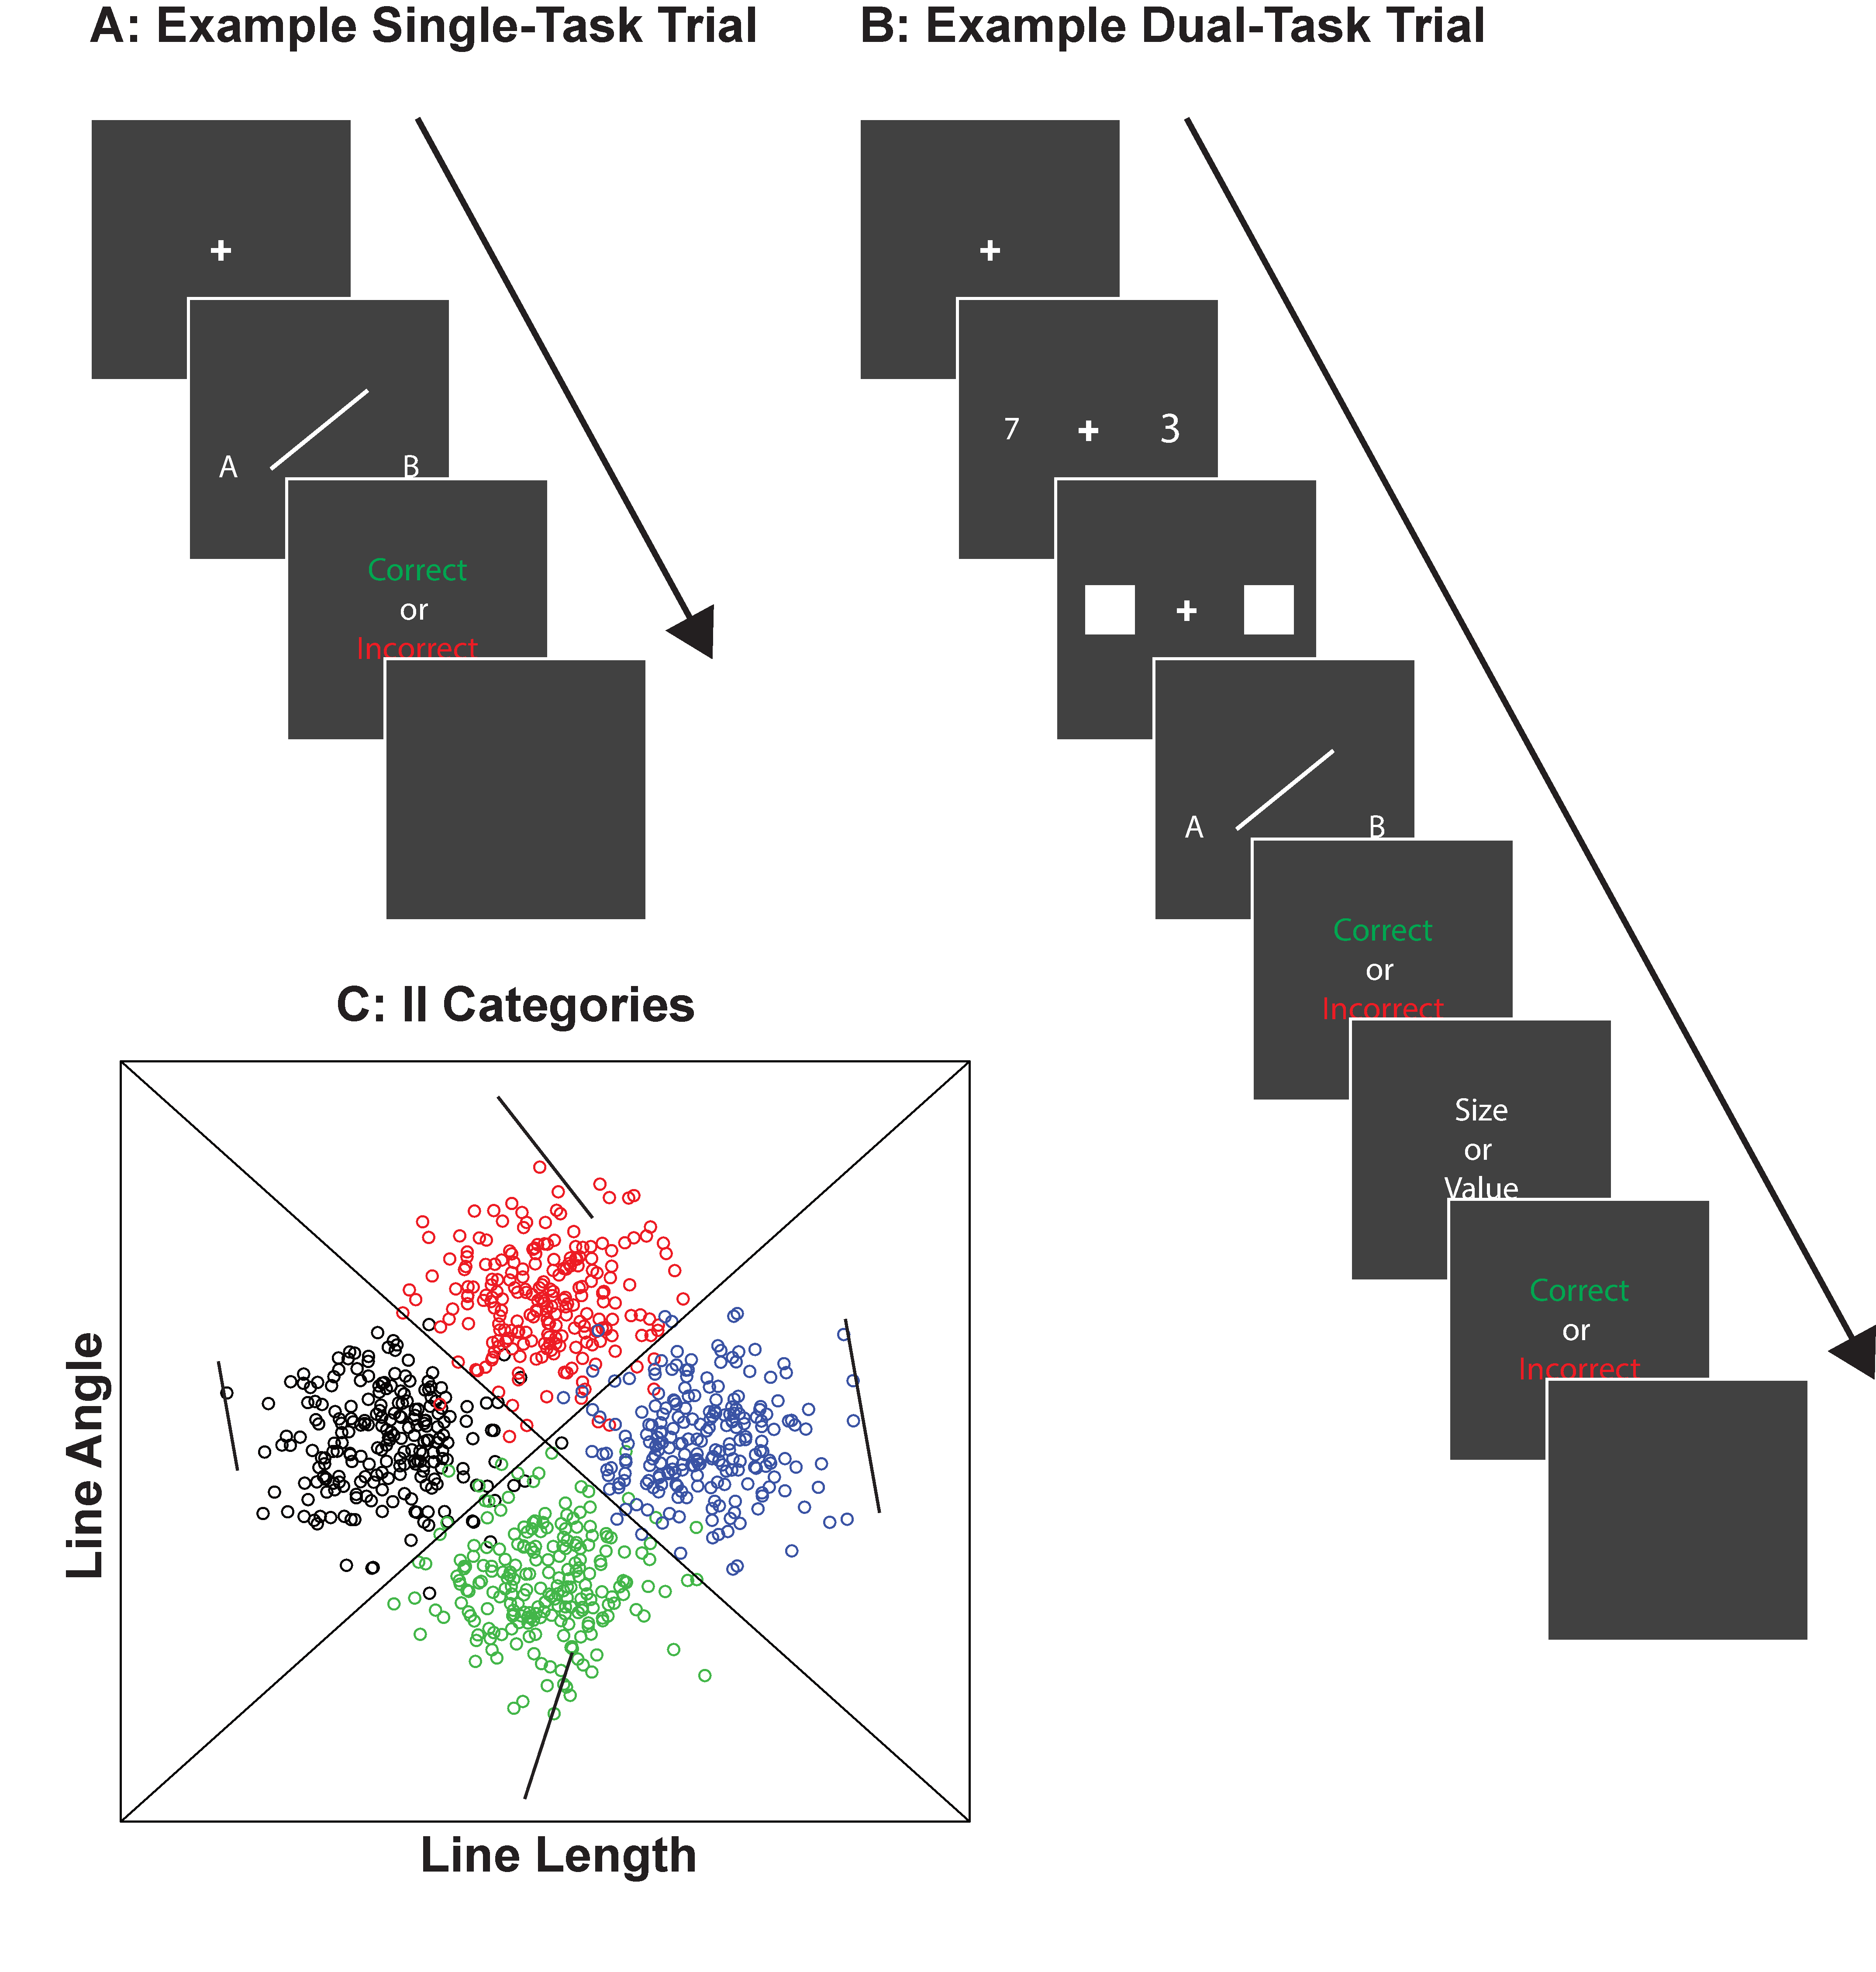
\includegraphics[width=1.0\textwidth]{../figures/fig_trials.pdf}
  \caption{ \textbf{A:} An Example trial during single-task conditions.
\textbf{B:} An example trial during dual-task conditions. \textbf{C:} The II
categories used during the acquisition phase of Crossley et al. (2013). }
  \label{fig:test_cats}
\end{figure}

Operationally, we require two conditions to conclude that unlearning is
successful: (1) the behavior disappears during the intervention, (2) both
relearning and new learning occur at the same rate as initial learning. In
contrast, if the learned information is preserved during the intervention, then
relearning the original categories should be faster than initial acquisition and
learning of new categories should be slower (because of interference).

The changes in feedback used during the intervention phase were chosen by
considering classic models of SR learning (panel A of Figure \ref{fig:models}).
These models assume that SR associations are learned at cortical-striatal
synapses via DA-dependent synaptic plasticity. Consistent with the classic view
that SR associations are robust against forgetting (e.g., we never forget the SR
associations involved in riding a bike), simply removing feedback during
intervention did not cause any substantial performance change (data not shown).
Therefore, an intervention phase with completely random feedback was used (i.e.,
correct feedback was randomly given 25\% of the time). Classic models predict
that this intervention will replace initially acquired S-R associations with
random strengths, thereby leading to identical or attenuated performance during
the test phase in both the Relearning and the New-Learning conditions. Contrary
to this prediction, random-feedback did not disrupt category knowledge. During
the test phase, performance relative to initial acquisition was enhanced in the
Relearning condition, and attenuated in the New-Learning condition; both
suggesting savings (left panel of Figure \ref{fig:unlearning_data}).

\begin{figure}[h]
\centering 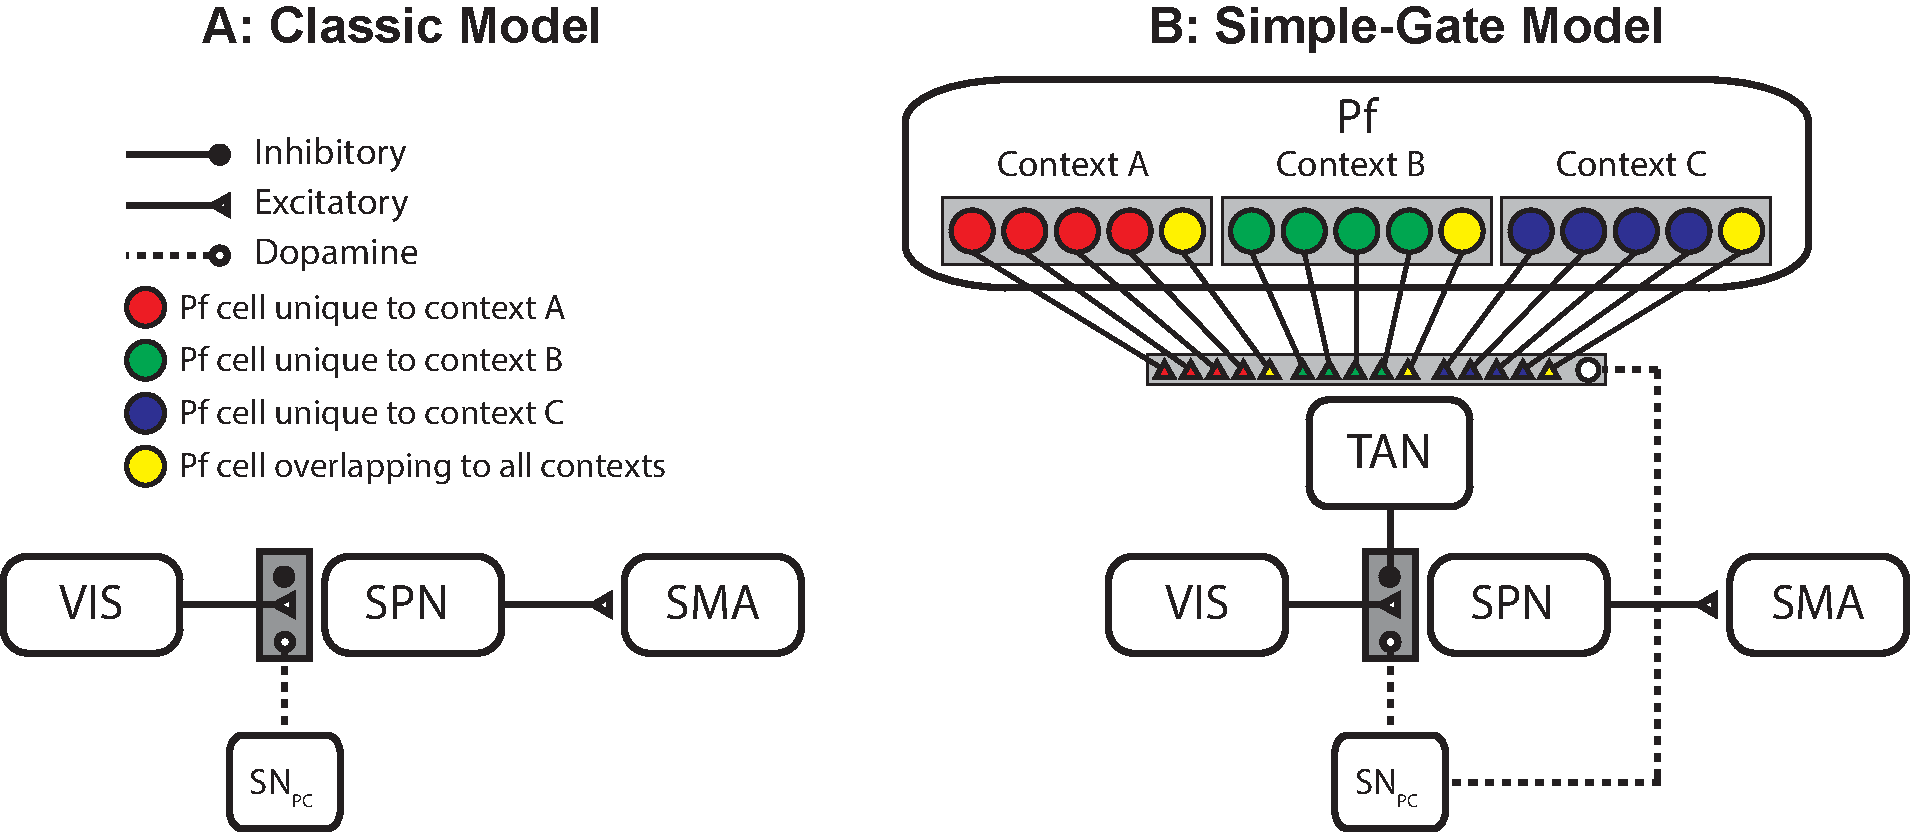
\includegraphics[width=1.0\textwidth]{../figures/fig_models.pdf}
  \caption{ \textbf{A: The Classic Model.} A classic model of procedural
learning based on a greatly simplified representation of the ``direct pathway''
through the basal ganglia. S-R associations are learned at cortical-striatal
synapses, which are modified via dopamine-dependent reinforcement learning. The
likelihood of repeating actions that lead to \emph{unexpected} positive outcomes
is gradually increased, and the likelihood of repeating actions that lead to
\emph{unexpected} negative outcomes is gradually decreased. \textbf{B: The TANs
Model.} The classic model of procedural learning with the addition of a
context-specific Pf-TAN pathway. This pathway acts as a gate on
cortical-striatal synaptic plasticity, permitting or preventing the learning and
expression of procedural knowledge. (MSN - medium spiny neuron of the striatum.
D1 - Direct pathway MSN expressing the D1 DA receptor. D2 - Indirect pathway MSN
expressing the D2 DA receptor. SMA - Supplementary Motor Area. SNpc - substantia
nigra pars compacta. Pf - parafascicular nucleus of the thalamus. VIS - visual
cortex)}
  \label{fig:models}
\end{figure}

The random feedback intervention result implies that \textit{there is a gating
mechanism that protects procedural learning from modification during random
feedback.} One candidate biological system for this gating mechanism is the
striatal cholinergic interneurons called TANs (for Tonically Active Neurons). It
is thought that these neurons mediate cortical-striatal synaptic plasticity via
presynaptic inhibition of cortical inputs to the striatum (Figure
\ref{fig:models}). As their name suggests, the TANs are tonically active in
their default state; however, they learn to pause their firing when stimuli that
predict reward are encountered. This allows striatal neurons to respond to
cortical input, and cortical-striatal learning to take place. The TANs are
driven by the parafascicular (Pf) nucleus in the thalamus, which signals salient
environmental cues; their pause response occurs only when the Pf-TAN synapse is
strong. The learning at both Pf-TAN synapses and cortical-striatal synapses is
driven by the DA reinforcement signal.

An updated procedural learning model that includes the TAN gating mechanism has
been shown to account for a variety of behavioral and physiological data from
simple instrumental conditioning tasks \cite{ashby_computational_2011,
crossley_expanding_2016}, including rapid relearning following extinction.
However, the model failed to account for the random feedback results described
above. This failure stems from the way DA activity was modeled. In the model, DA
firing reflected a reward prediction error (RPE; which equals the difference
between the obtained and expected outcomes), and since random feedback is
\emph{by definition} completely unpredictable, the model predicted persistent
RPEs and corresponding DA fluctuations during random feedback. These
fluctuations prevented the TANs from closing the gate on cortical-striatal
plasticity, and thereby permitted random feedback to disrupt initial learning.

In order for the TANs to reliably close the gate and protect cortical-striatal
plasticity during random feedback, two conditions must be met:

\begin{description}
\item \textit{1. The model must detect when feedback has become random.} Random
feedback has several properties, but our results suggest that the most critical
-- at least with respect to learning and unlearning -- is that random feedback
is non-contingent on action. More specifically, when the feedback is random the
correlation between response confidence and feedback valence is zero. This
correlation, which we refer to as \textit{feedback contingency}, is a critical
requirement of successful learning. For example, \citeA{AshbyVucovich2016}
compared learning under high- and low-levels of feedback contingency in two
different category-learning tasks -- one that recruits declarative memory and
one that recruits procedural memory. In both tasks, the high- and
low-contingency conditions used exactly the same stimuli, had exactly the same
optimal strategies, and optimal accuracy was 80\% correct in all conditions. The
results were virtually identical in the two tasks. Learning was good when
feedback contingency was high, but degrading feedback contingency seemed to
abolish all learning in most participants.

\item \textit{2. The TANs must close the gate when non-contingent (e.g., random)
feedback is detected.} This only occurs when Pf-TAN synapses undergo consistent
weakening (see Figure \ref{fig:models}B). This was modeled in
\cite{crossley_erasing_2013} by assuming that the magnitude of \textit{the DA
response is attenuated and biased below baseline when feedback contingency is
low.}
\end{description}

With this modification to the DA system, the model not only accounts for savings
in relearning after random feedback intervention, but also makes a novel
prediction: \textit{Mixed feedback that contains some random and some veridical
feedback trials produces an intermediate level of contingency and therefore
should prevent the TANs from completely closing the gate on cortical-striatal
plasticity, thereby enabling modification of initial learning.} Our results
supported this prediction (panel B of Figure \ref{fig:unlearning_data}) -- that
is, performance during the Test phase was identical in the Relearning and
New-Learning conditions, and each was significantly different from initial
learning.

One potential confound of this mixed-feedback intervention was that the rate of
positive feedback was greater than during the random-feedback intervention (note
the different accuracy levels during the intervention phase in panels A and B of
Figure \ref{fig:unlearning_data}). To address this confound, Crossley et al.
(2013) examined performance with an intervention that included random feedback,
but with a positive feedback rate of 40\%. This intervention increased the
overall positive feedback rate, but since it was entirely random, feedback
contingency was still zero. The results from this experiment are shown in panel
C of Figure \ref{fig:unlearning_data}, and are virtually identical to our
original random feedback intervention (where the positive feedback rate was
25\%, see panel A, Figure \ref{fig:unlearning_data}). Thus, mixed feedback
intervention may constitute an effective intervention for procedural
modification.

\begin{figure}[h]
\centering 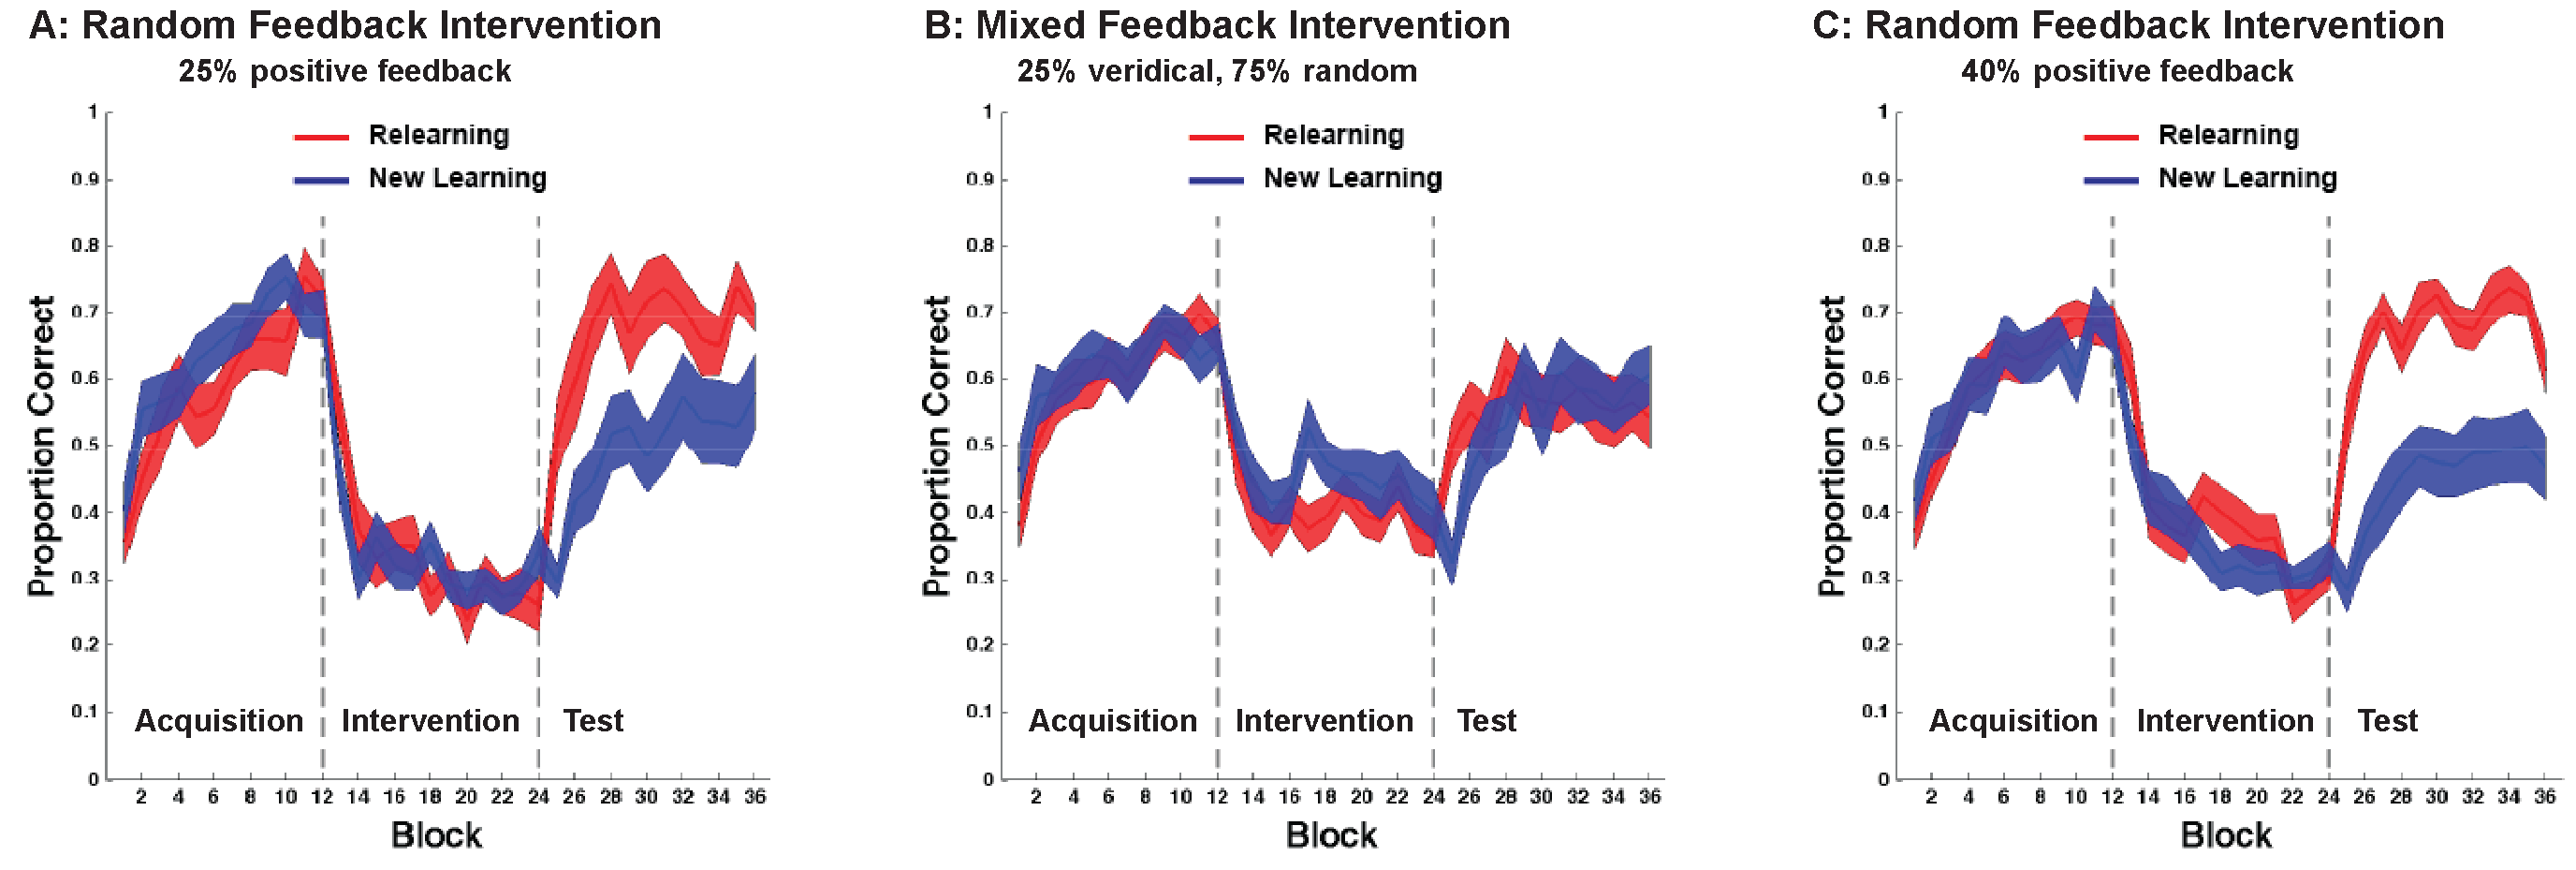
\includegraphics[width=1.0\textwidth]{../figures/fig_unlearning_results.pdf}
  \caption{ Behavioral results with different interventions. \textbf{A:} Random
feedback intervention with 25\% positive feedback. Accuracy drops to near chance
during intervention, but is reacquired faster than original learning in the
Relearning condition (red). In contrast, a lasting interference is observed in
the New Learning condition (blue). Both results are consistent with the
hypothesis that initial learning was not overwritten by random feedback.
\textbf{B:} Mixed feedback intervention. Accuracy drops during intervention --
though not to chance (i.e., 25\%) -- but subsequent learning proceeds at
approximately the same rate and to the same extent as initial learning when
either the original category-response mappings (red) or new category-response
mappings (blue) are introduced. These results are consistent with the hypothesis
that initial learning was overwritten during the intervention. \textbf{C:}
Random feedback intervention with 40\% positive feedback. Results are
qualitatively identical to random feedback intervention with 25\% positive
feedback, implying that the mixed feedback results were driven by feedback
contingency and not by positive feedback. }
  \label{fig:unlearning_data}
\end{figure}

Crossley et al. (2013) hypothesized that the gate on procedural learning --- and
therefore the key to procedural modification --- is controlled by the degree of
feedback contingency. Even so, we made no predictions about how contingency is
computed by the nervous system. This article begins addressing this question --
by asking whether feedback contingency is computed via declarative mechanisms
(e.g., prefrontal networks involved in working memory and executive reasoning).
Our rationale is as follows: If feedback contingency is estimated by declarative
mechanisms, then increasing cognitive load during the intervention phase (by
requiring participants to simultaneously perform a dual task) should impair the
ability of participants to detect a change to random feedback, which should
cause the TANs gate to remain open, thereby allowing random feedback to modify
the procedural knowledge that was acquired during initial learning.

With this goal in mind, we performed an experiment that mimicked the design of
Crossley et al. (2013), except we added a concurrent numerical Stroop task
during key classification trials. Previous research suggests that this dual task
interferes with category learning that recruits declarative memory but not with
category learning that recruits procedural memory \cite{WaldronAshby2001}. Thus,
since our categorization task recruits procedural memory, any effect of the dual
task on categorization performance should be due to its effects on contingency
estimation, rather than on category learning per se.

In conditions 1 -- 3, the first dual-task trial was 50 trials before the onset
of intervention, and continued for 100, 200, or 300 trials, respectively. In
Condition 4, the first dual-task trial was 50 trials after the onset of
intervention, and continued for 250 trials. Comparing conditions 1 -- 3 to
condition 4 will allow us to assess the importance of disrupting the estimation
of feedback contingency during the transition from acquisition to intervention.
Condition 5 was a control condition in which no concurrent Stroop task was ever
performed.

If feedback contingency estimation depends on declarative mechanisms then two
behavioral markers are expected: (1) the dual task should slow the drop in
categorization accuracy that occurs with the onset of random feedback; and (2)
reacquisition of the original category learning should be slower in the dual
task conditions than in the no dual-task control.

\section*{Methods}
\subsection*{Design} There were four dual-task conditions (Condition 1 -- 4) and
one no dual-task control condition (Condition 5). The dual-task conditions
differed on two dimensions, (1) the number of trials on which the dual task was
applied, and (2) whether or not the onset of the dual task preceded the onset of
intervention.

\subsection*{Participants} 163 participants were recruited from the University
of Texas at Austin undergraduate population. There were 30 participants in
Condition 1, 34 participants in Condition 2, 32 participants in Condition 3, 33
participants in Condition 4, and 34 participants in Condition 5. All
participants completed the study and received course credit for their
participation. All participants had normal or corrected-to-normal vision.

\subsection*{Stimuli and Categories} Stimuli were black lines that varied across
trials only in length (pixels) and orientation (degrees counterclockwise
rotation from horizontal). The stimuli are illustrated graphically in Figure 1,
and were identical to those used by Crossley et al. (2013).

\subsection{Procedure} Participants in all conditions were told that they were
to categorize lines on the basis of their length and orientation, that there
were four equally-likely categories, and that high levels of accuracy could be
achieved. The experiment included three phases: acquisition (300 trials),
intervention (400 trials), and reacquisition (150 trials). During acquisition
and reacquisition, feedback was based on the participant's response, whereas
feedback was random during the intervention. Participants were given no prior
instructions about the phases, and the transition from one phase to another
occurred without any warning to the participant.

At the start of each non-Stroop trial, a fixation point was displayed for 1
second and then the stimulus appeared. The stimulus remained on the screen until
the participant generated a response by pressing the ``Z'' key for category
``A'', the ``W'' key for category B, the ``/'' key for category C, or the ``P''
key for category D. Written instructions informed participants of the category
label to button mappings. An ``invalid key'' message was displayed if any other
button was pressed. The word ``Correct'' was presented for 1 second if the
response was correct or the word ``Wrong'' was presented for 1 second if the
response was incorrect (except during the intervention phase in which feedback
was completely random).

Stroop trials began with a fixation point that was displayed for 1 second. The
category stimulus and the Stroop stimuli (numbers flanking the category
stimulus) were displayed simultaneously. After 200 ms the Stroop stimuli were
replaced by white rectangles which remained on the screen until they made a
category response. Responses emitted before the Stroop stimuli were replaced by
white rectangles were not accepted. Feedback about the category response was
given immediately in the same fashion as on non-Stroop trials. The word
``value'' or ``size'' then appeared on the screen prompting participants to
indicate which side contained the numerically larger or the physically larger
number. Participants pressed the ``F'' key to choose the number on the left or
the ``J'' key to choose the number on the right. The word ``Correct'' was then
again presented for 1 second if the response to the Stroop task was correct or
the word ``Wrong'' was presented for 1 second if the response was incorrect. See
Figure 1 for example trials both including and excluding the Stroop component.
The Stroop task was included on trials 251-350 in condition 1, 251-450 in
condition 2, 251-550 in condition 3 and 400-650 in condition 4.

Participants were instructed to try their hardest on both task components but to
prioritize performance on the Stroop task. Both the category-learning task and
the Stroop task were explained to participants prior to beginning the
experiment, and on screen messages warned them when the Stroop component would
begin, and again when it would end. These messages read, ``You will now perform
both the categorization task and the paired numbers task simultaneously. Keep
trying your hardest!'' and ``You have now finished the section with the paired
numbers task. You will now be shown only the line categorization task. Keep
trying your hardest.'' 85\% of Stroop trials the numerically larger number was
physically smaller. The proportion of Stroop trials that prompted ``size'' or
``value'' was split 50/50. Accuracy on the numerical Stroop task was indicated
at the top of the screen when they received feedback regarding their performance
on the concurrent task on each trial. This score was displayed in green if it
was above 80\% and red if it was below 80\%. Note that when we refer to the
``dual-task'', we are referring to the Stroop task just described.

\section*{Results}
\subsection*{Numerical Stroop Accuracy}
\begin{figure}[t]
\centering 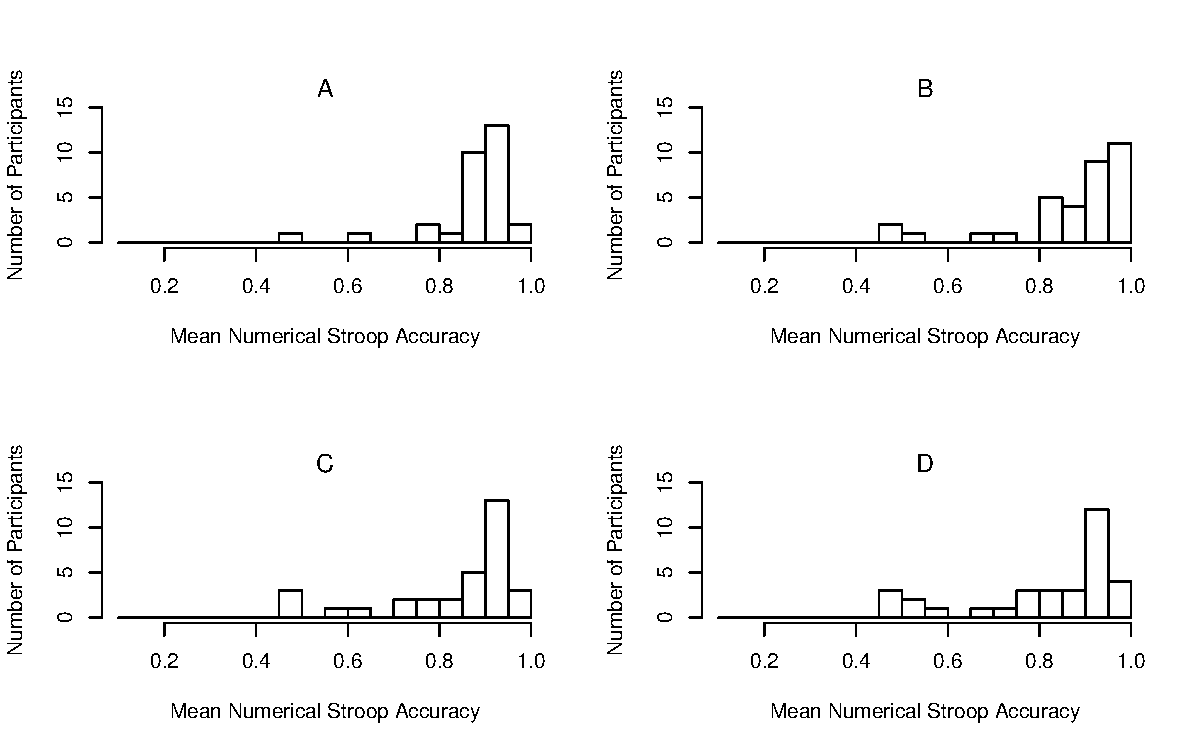
\includegraphics[width=1.0\textwidth]{../figures/fig_exc_dual.pdf}
    \caption{ Histograms showing distribution of mean Numerical Stroop accuracy
seperately for each condition. \textbf{A:} Condition 1. \textbf{B:} Condition 2.
\textbf{C:} Condition 3. \textbf{D:} Condition 4. }
    \label{fig:exc_dual}
\end{figure}

Figure \ref{fig:exc_dual} shows histograms characterizing mean dual-task
performance seperately for each condition. Overall, mean accuracy on the
dual-task was very good, with mean proportion correct at $0.88$ in Condition 1,
$0.87$ in Condition 2, $0.84$ in Condition 3, and $0.82$ in Condition 4.

\subsection*{Classification Accuracy}
\begin{figure}[t]
\centering 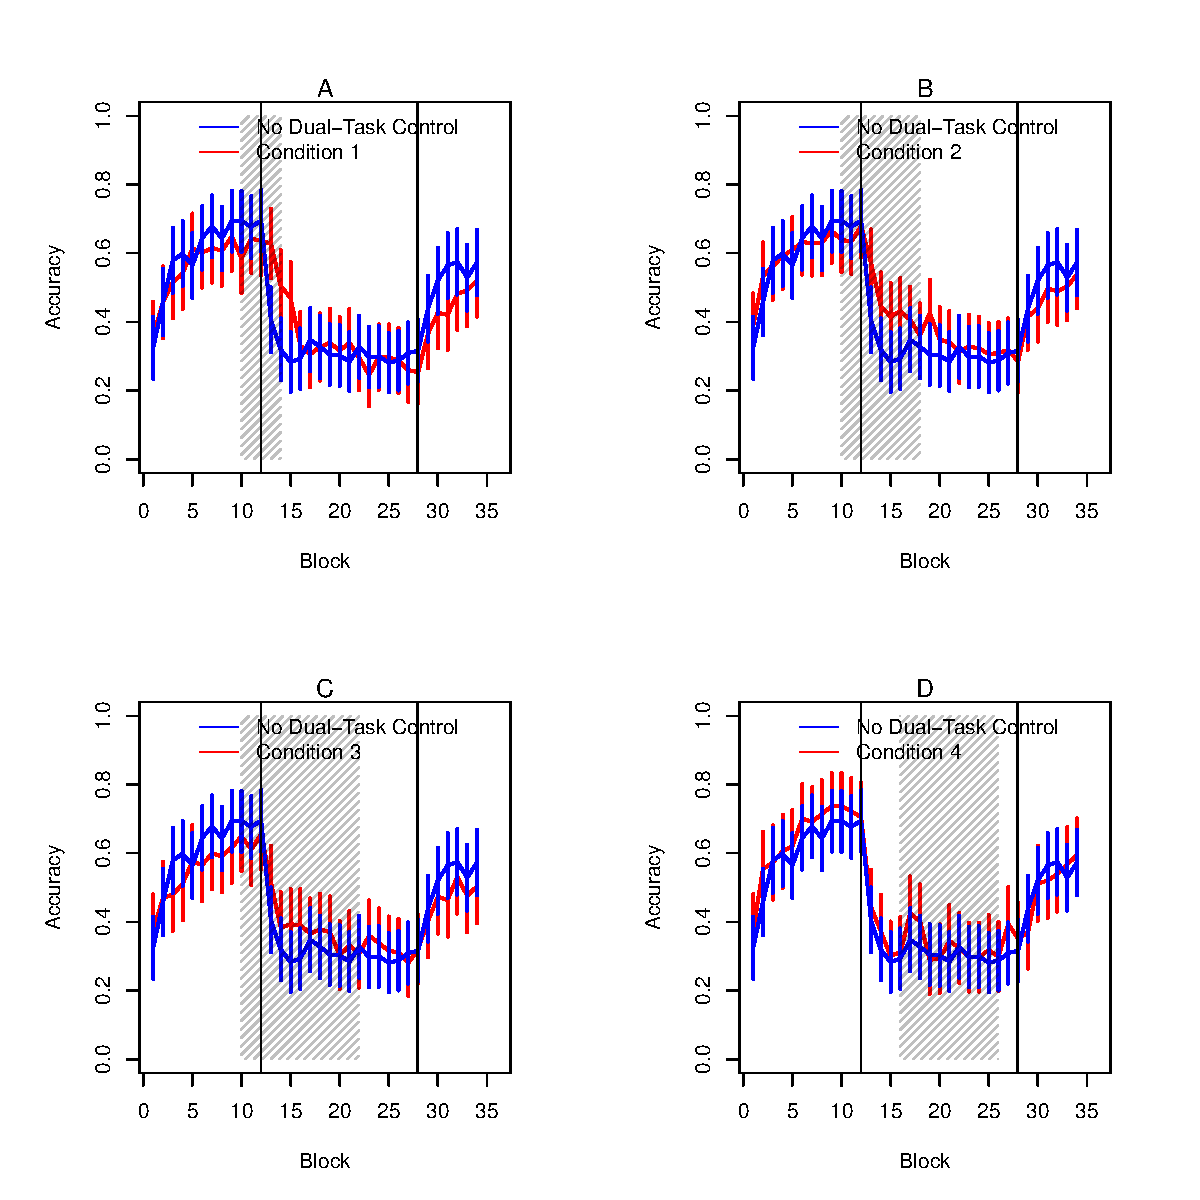
\includegraphics[width=1.0\textwidth]{../figures/fig_learning_curves.pdf}
  \caption{ Mean accuracy per 25 trial block. The blue line in each panel is
Condition 5 (no dual-task control). The hatch marks indicate dual-task trials.
The key features are (1) dual-task slows the change in classification strategy
(seen in this plot as ``accuracy'' decline), and (2) the dual-task conditions
show less savings than the no dual-task control. There is no obvious
dose-dependent effect of the dual task, nor is there an obvious difference
between dual-task conditions. \textbf{A:} Condition 1 (dual-task applied on
trial 251 through trial 350). \textbf{B:} Condition 2 (dual-task applied on
trial 251 through trial 450). \textbf{C:} Condition 3 (dual-task applied on
trial 251 through trial 550). \textbf{D:} Condition 4 (dual-task applied on
trial 351 through trial 650). Error bars are SEM. }
  \label{fig:learning_curves}
\end{figure}

Figure \ref{fig:learning_curves} shows the mean accuracy in each block of 25
trials across the duration of the experiment. Recall that if feedback
contingency is estimated via declarative mechanisms, then (1) dual-task trials
should slow the change in classification performance during intervention, and
(2) dual-task conditions should show reduced savings relative to the no
dual-task control. We see evidence for both features in our data.

\subsubsection*{Acquisition} Conditions 1 -- 5 are identical for the first 250
trials (10 blocks) of acquisition (before dual-task onset), and so we expect
performance during these blocks to be the same across conditions. This is
clearly the case by visual inspection of Figure \ref{fig:learning_curves}, and
is supported by the results of a 5 Condition $\times$ 10 Block repeated-measures
ANOVA. The main effect of Condition was nonsignificant [$F(4,1620) = 1.89, p =
0.11, \Omega^2 = 0.00$], and so was the Condition $\times$ Block interaction
[$F(4,1620) = 1.08, p = 0.37, \Omega^2 = 0.00$]. However, there was a
significant effect of Block [$F(1,1620) = 191.00, p < 0.001, \Omega^2 = 0.10$],
reflecting improvement across the acquisition phase.

\subsubsection*{Intervention} If the estimation of feedback contingency depends
on declarative mechanisms, then we expect change in performance during
intervention to be slowed during the simultaneous performance of the dual task.
This is clearly seen in Figure \ref{fig:learning_curves}, and is supported by
the results of a 5 condition $\times$ 14 block repeated-measures ANOVA. A
significant effect of Condition [$F(4,2598) = 9.74, p = 0.00, \Omega^2 = 0.01$]
reflected an overall difference in intervention performance in dual-task
conditions relative to the no dual-task control. A significant effect of Block
[$F(1,2598) = 166.65, p < 0.001, \Omega^2 = 0.06$] reflected the change in
classification performance across intervention seen in all conditions. The
Condition $\times$ Block interaction was also significant [$F(4,2598) = 14.64, p
< 0.001$, $\Omega^2 = 0.02$], reflecting the slower change in performance in the
dual-task conditions relative to the no dual-task control.

The directional interpretation of the omnibus tests is supported by several
planned comparisons on the overall mean accuracies during the intervention
phase. First, intervention accuracy in all dual-task conditions was
significantly different from intervention accuracy in the no dual-task control
[condition 1 > condition 5: $t(940) = 2.78$, $p < .05, d = 0.25$; condition 2 >
condition 5: $t(1046) = 5.31, p < .01, d = 0.87$; condition 3 > condition 5:
$t(962) = 5.45, p < .01, d = 0.96$; condition 4 > condition 5: $t(996) = 2.99$,
$p < .01, d = 0.28$]. Second, the dual task slowed the accuracy drop during
intervention only in conditions in which it was first introduced during the
acquisition phase [condition 2 > condition 4: $t(1063) = 1.94, p = 0.05, d =
0.12$; condition 3 > condition 4: $t(1037) = 2.24$, $p = 0.03, d = 0.16$],
although this difference was not observed in condition 1 (shortest dual-task
exposure) [condition 1 > condition 4: $t(1006) = -0.23$, $p = 0.82, d = 0.00$].

\subsubsection*{Savings: Group Level}
\begin{figure}[t]
\centering 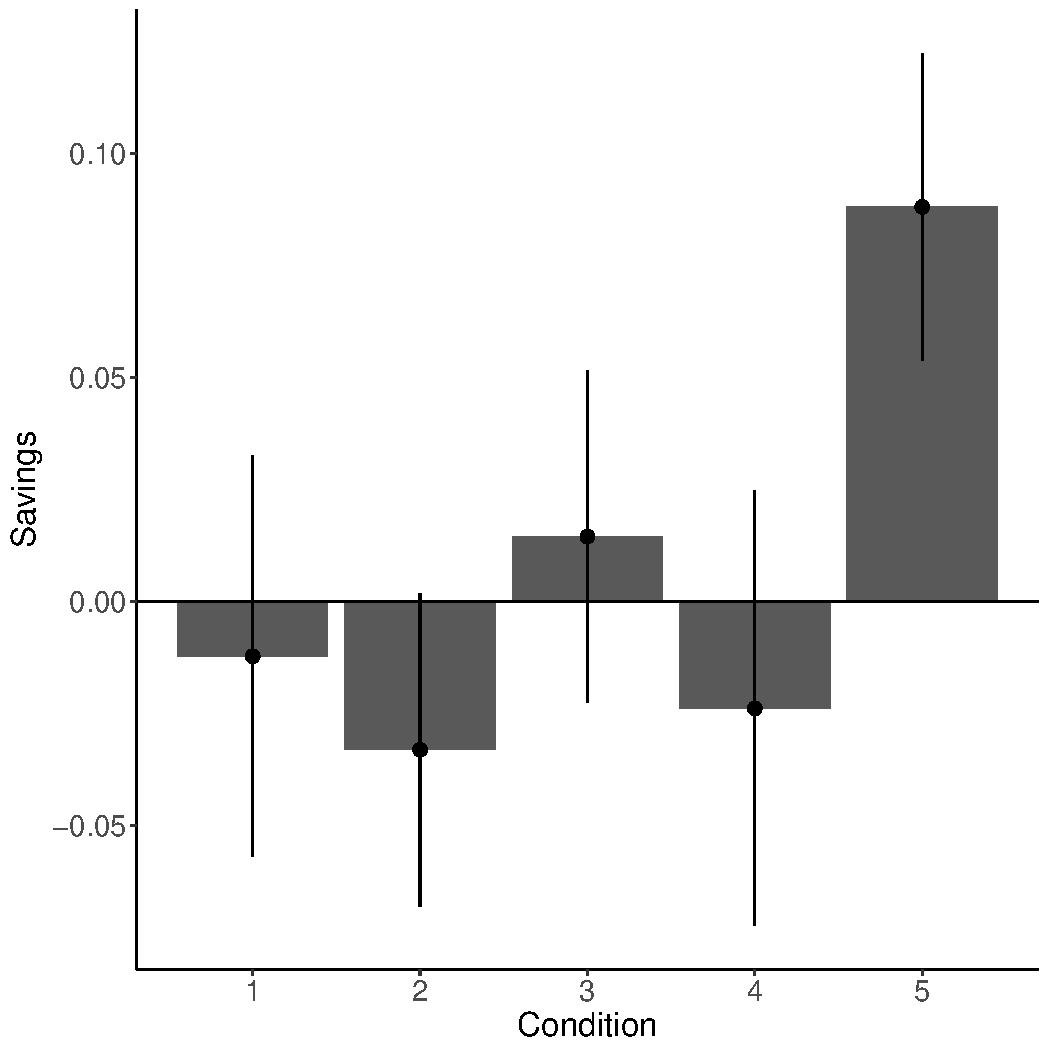
\includegraphics[width=1.0\textwidth]{../figures/fig_savings.pdf}
  \caption{ savings (mean of all 150 reacquisition trials - mean of the first
150 acquisition trials) in all conditions of the present experiment, and also
including data from the random feedback condition of crossley et al. (2013),
which shows the savings observed in a no dual-task control condition with only
300 trials of intervention. Each circle corresponds to a single participant. }
  \label{fig:savings}
\end{figure}

\begin{figure}[t]
\centering 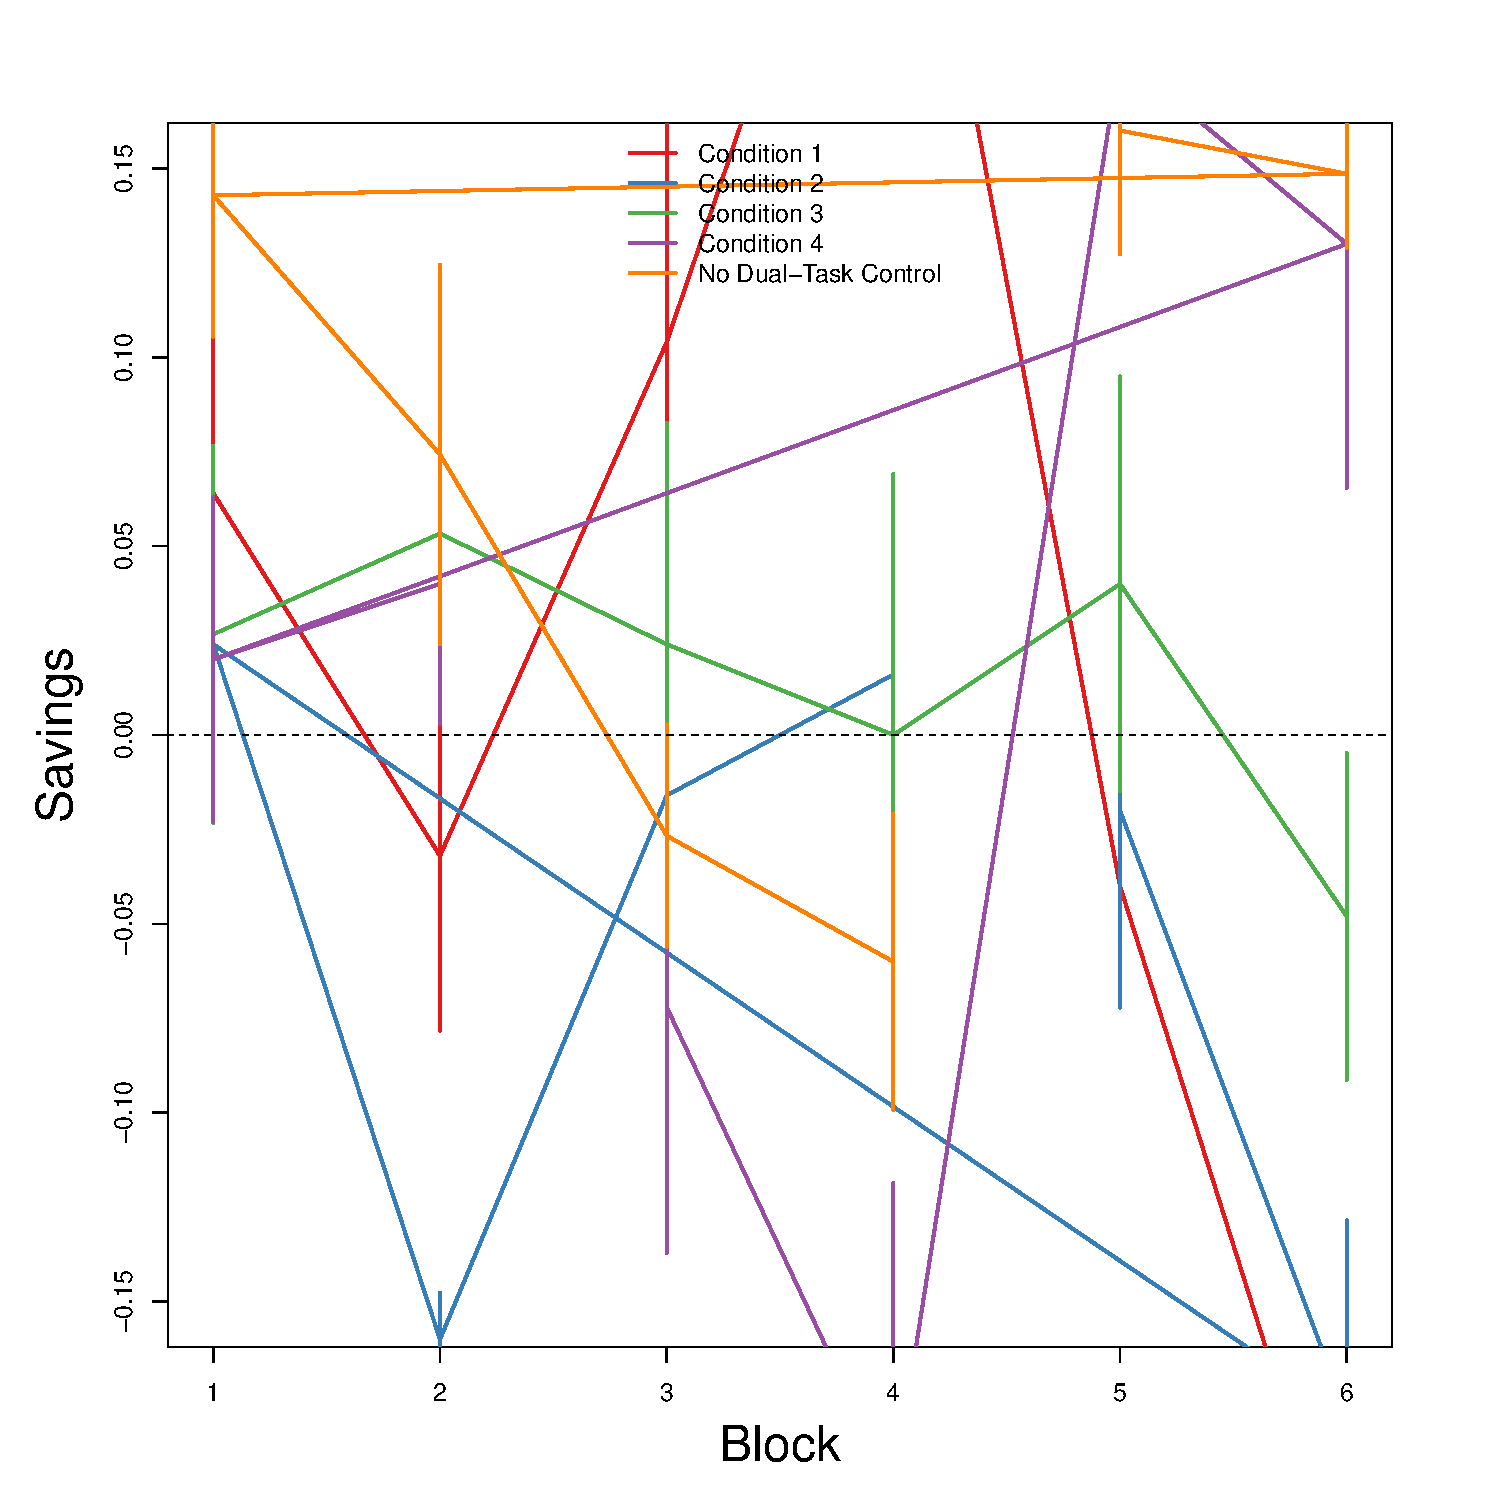
\includegraphics[width=1.0\textwidth]{../figures/fig_savings_per_block.pdf}
  \caption{ Savings (reacquisition - acquisition) per 25 trial block. Error bars
are SEM. }
  \label{fig:savings_per_block}
\end{figure}

If the computation of feedback contingency depends on declarative systems, then
we expect the dual-task conditions to exhibit less savings than the no dual-task
control -- that is, we expect reacquisition of the original categories to be
slower under dual-task conditions. This is apparent via visual inspection of
Figure \ref{fig:learning_curves} (e.g., the red lines are always below the blue
line), and also of Figure \ref{fig:savings}, which shows the savings observed
for every participant in every condition as a box plot with individual
participant data points superimposed. As a comparison, Figure \ref{fig:savings}
also shows the results from the random-feedback intervention condition of
Crossley et al. (2013), which was similar in design to our no dual-task control
condition (although the Crossley et al. condition included fewer intervention
trials).

Figure \ref{fig:savings_per_block} shows the savings during each 25-trial block,
where savings is defined as reacquisition accuracy minus acquisition accuracy on
the block in the same ordinal order (e.g., first reacquisition block accuracy
minus first acquisition block accuracy, etc.). Several features of these data
are worth noting. First, savings in the no dual-task control condition is
uniformly greater than in any other condition. Second, there is little
difference in savings in any dual-task condition. Third, in every condition, the
curves are decreasing, and fourth, in every case, savings become negative,
indicating that asymptotic accuracy during reacquisition was lower than during
acquisition in every condition.

These observations are supported via the results of a 5 condition $\times$ 6
block ANOVA. There was a significant effect of Condition [$F(1,974) = 5.77, p <
0.05, \Omega^2 = 0.01$], indicating less savings in the dual-task conditions
relative to the no dual-task condition. There was a significant effect of Block
[$F(1,974) = 22.55, p < 0.001, \Omega^2 = 0.02$], indicating that savings in all
conditions was most prominent during early blocks and gradually decreased (see
Figure \ref{fig:savings_per_block}). The Condition $\times$ Block interaction
was n.s. [$F(1,974) = 0.001$, $p = 0.97, \Omega^2 = 0.00$].
    
The directional interpretation of these omnibus tests is supported by several
planned comparisons. First, Condition 2 savings were significantly less than in
the no dual-task control condition [$t(63) = 2.09, p = 0.04, d = 0.55$], whereas
savings in the other dual-task conditions were all marginally less than in the
control condition [condition 1 < control: $t(46) = -1.24, p = 0.22, d = 0.22$;
condition 3 < control: $t(57) = -1.63, p = 0.11, d = 0.35$; condition 4 <
control: $t(61) = -1.67, p = 0.10, d = 0.36$]. Second, there were no significant
differences in savings between any dual-task conditions \footnote{Note that the
following p-values should all be corrected for multiple comparisons. However,
any such correction would only increase each p value, and therefore would not
change our nonsignificance conclusions.} [condition 1 > condition 2: $t(53) =
0.37, p = 0.71, d = 0.02$; condition 1 > condition 3: $t(56) = 0.12, p = 0.90, d
= 0.00$; condition 1 > condition 4: $t(53) = 0.08, p = 0.94, d = 0.00$;
condition 2 > condition 3: $t(63) = -0.29, p = 0.78, d = 0.01$; condition 2 >
condition 4: $t(65) = -0.36, p = 0.72$, $d = 0.02$; condition 3 > condition 4:
$t(62) = -0.06, p = 0.96, d = 0.00$].

\subsubsection*{Participant-Level Savings}
\begin{figure}[t]
\centering 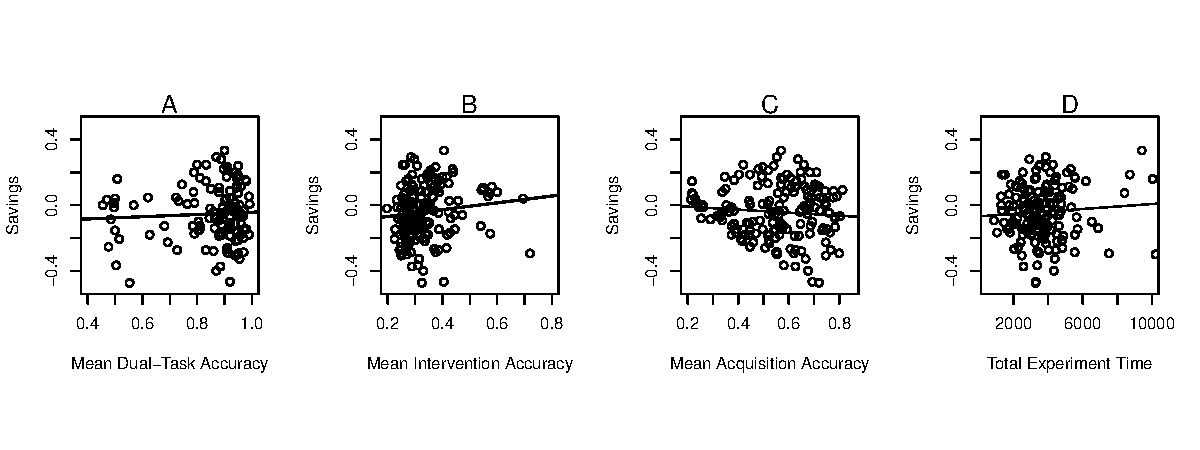
\includegraphics[width=1.0\textwidth]{../figures/fig_save_mixed_2.pdf}
  \caption{ Regression analyses to examine possible predictor variables for
savings. A: Mean dual-task accuracy. B: Mean Intervention accuracy. C: Mean
acquisition accuracy. D: Total experiment time. }
  \label{fig:savings_mixed}
\end{figure}

Figure \ref{fig:savings} shows large individual differences -- with many
participants in all conditions expressing both positive and negative savings. To
examine these differences in more detail, we performed an exploratory analysis
that examines what factors might predict savings in individual participants. In
particular, we performed a multiple regression with three predictors: (1) mean
dual-task accuracy, (2) mean intervention accuracy, and (3) mean acquisition
accuracy. Dual-task performance might reflect the degree to which the
computation of feedback contingency is impaired, and thereby predict savings.
Mean intervention accuracy may reflect the degree to which procedural knowledge
is being expressed, and therefore is vulnerable to modification. Mean
acquisition accuracy may predict savings in that the stronger the initial
learning, the more robust to intervention it may be, and the more likely it
should be manifest as savings in relearning.

Figure \ref{fig:savings_mixed} plots savings against each of these predictor
variables. Note that data was pooled across the four dual-task conditions for
this analysis. The regression revealed a significant negative coefficient for
mean acquisition performance [$\beta=-0.23$, $t(125)=-2.17$, $p<.05$], showing
that the better a participant did during acquisition, the less savings they were
likely to express. The coefficient for mean intervention performance was
positive and nearly significant [$\beta=.30, t(125)=1.79, p=.07$], showing that
there was a trend for higher intervention accuracy to predict better savings.
The coefficient for mean dual-task performance was not significantly different
from zero [$\beta=.09, t(125)=.87$, $p=.39$]. The overall model, however, was
not a good predictor of savings, accounting for only 5\% of the total variance
in the data [$r^2=.05, F(3,125)=2.29, p=.08$].

% \subsection*{Decision-Bound Modeling}
% \begin{figure}[t] %
\centering 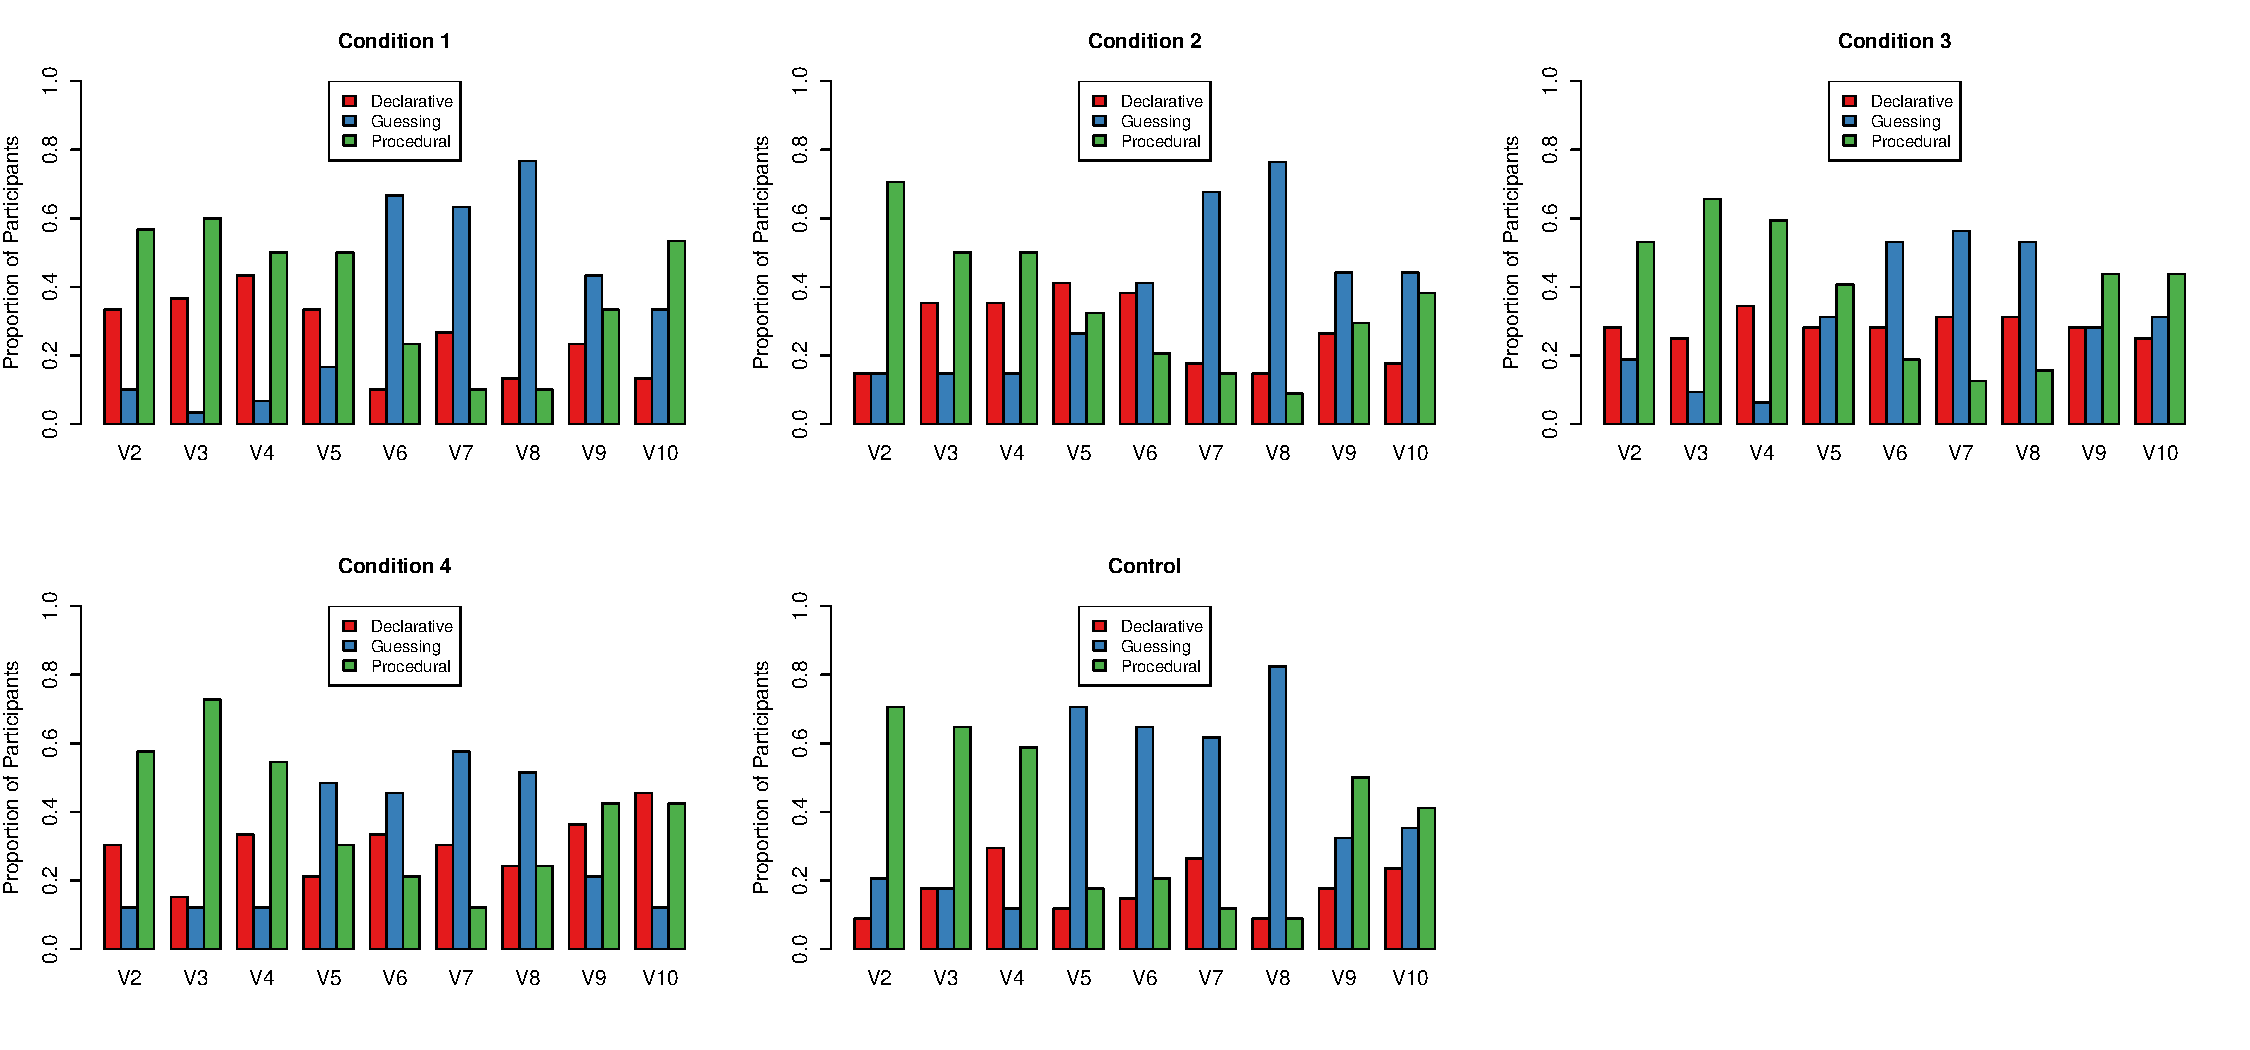
\includegraphics[width=1.0\textwidth]{../figures/fig_model_fits.pdf}
% \caption{ % Proportion of participants best fit by a decision-bound model
assuming a % procedural, declarative, or guessing strategy. The key feature of
this % figure is that participants in the no dual-task control condition changed
% their response strategy more during the intervention more quickly than %
participants in all dual-task conditions. % \textbf{A:} Condition 1 (dual-task
applied on trial 251 through trial 350). % \textbf{B:} Condition 2 (dual-task
applied on trial 251 through trial 450). % \textbf{C:} Condition 3 (dual-task
applied on trial 251 through trial 550). % \textbf{D:} Condition 4 (dual-task
applied on trial 351 through trial 650). % \textbf{E:} Condition 5 (no dual-task
control). % }
% \label{fig:exp_fits}
% \end{figure}

\section*{Discussion}
\subsection*{Summary}
Feedback contingency, which we define as the correlation between response
confidence and feedback valence, can be manipulated experimentally by varying
the randomness of feedback. Our current and previous results
\cite{crossley_erasing_2013} suggest that such manipulations may be key to
flexibly modifying procedural memories. To our knowledge, this article reports
results from the first behavioral experiments that investigate the cognitive and
neural mechanisms that estimate feedback contingency. Specifically, our goal was
to determine whether prefrontal-based declarative memory mechanisms mediate
contingency estimation. If they do, then a dual task that depends on working
memory and executive function should make it more difficult for participants to
recognize the sudden onset of random feedback. In our experiments, behavioral
signatures of this difficulty would include (1) a slowed decrease in
classification accuracy during intervention, and (2) decreased savings in
relearning relative to a no dual-task control. Our results were consistent with
both of these predictions.

\subsection*{Weakness of Raw Savings} Perhaps our most conspicuous and
unanticipated result was the lack of large and robust savings in any condition.
Even in the no dual-task control, savings is only clearly expressed during early
blocks of reacquisition -- that is, during the first two blocks of
reacquisition, performance was better than during initial acquisition, but
during the last few blocks it was worse. We speculate that this is due to the
duration of the intervention phase, which was a full 100 trials longer than in
previous studies \cite{crossley_erasing_2013, CrossleyAshbyMaddox2014}. Does
this finding suggest that longer interventions are a possible key to true
unlearning? Several features of our data argue against this hypothesis. First,
participants in the no dual-task control condition showed considerable savings
during the first 50 trials (i.e., 2 blocks) of reacquisition (see Figure
\ref{fig:savings_per_block}). If the longer intervention caused unlearning then
such savings should not have occurred. Second, this initial savings is reversed
to an interference during the last half of the reacquisition phase. True
unlearning predicts zero savings throughout reacquisition. The most parsimonious
account of the negative savings that occurred in every condition during the
latter half of the reacquisition phase may be participant fatigue.

At first glance, one might therefore wonder whether all our results simply
reflect that categorization with a dual-task is more tiring than categorization
without a dual task. In other words, perhaps dual-task participants were more
fatigued than no dual-task control participants at the beginning of the
reacquisition phase, and this extra fatigue was the primary reason they did not
show savings, rather than because the intervention disrupted their acquisition
memory traces. However, a closer examination argues against this hypothesis.
First, and most importantly, all three conditions in which the dual-task
overlapped the transition from acquisition to intervention showed a slower
decrease in intervention accuracy than in either the no dual-task control
condition or in Condition 4, where the dual task did not begin until later
during intervention (see Figure 5). Thus, one important signature of unlearning
appeared in Conditions 1 -- 3 early in the experiment (i.e., well before the
beginning of reacquisition), before fatigue should have been a factor. Second,
if participant fatigue was the driving factor, then there should be differences
among dual-task conditions, which we did not observe. Specifically, Condition 1
had the fewest dual-task trials and Conditions 3 and 4 had the most. So the
fatigue hypothesis should predict poorer reacquisition performance in Conditions
3 and 4 than in Condition 1. Figure \ref{fig:savings_per_block} disconfirms this
prediction. Third, we performed a linear regression (on the pooled data from all
five experimental conditions) that tried to predict savings as a function of
overall experiment time. The idea here is that the longer the experiment took,
the more susceptible the participant should be to fatigue, and the less savings
they should express. The coefficient for total experiment time was not
significantly different from zero [$\beta=7.5 \times 10^{-6}, t(161)=.93,
p=.35$], and did not predict a significant proportion of variance in savings
[$r^2=.005, F(1,161)=.87, p=.35$].

\subsection*{Category Learning as a Procedural Skill} A natural question for
readers unfamiliar with the category-learning literature is whether our
behavioral paradigm is a good choice for studying procedural behaviors. In other
words, how can a task with such simple motor demands (e.g., push a button)
possibly recruit procedural networks that are strongly tied to motor processes?
In fact, the empirical evidence is strong that performance improvements in the
classification task used here are mediated via procedural learning and memory. A
large database of evidence suggests that humans have multiple, qualitatively
distinct category-learning systems \cite{AshbyCOVIS1998, AshbyMaddox2005,
EricksonKruschke1998}, and according to this view, procedural memory is used to
form many-to-one stimulus-to-response mappings (S-R associations), whereas
declarative memory is used to apply rules and test explicit hypotheses about
category membership.

The majority of this evidence comes from prior research with rule-based (RB) and
information-integration (II) category-learning tasks \cite{HelieRoederAshby2010,
NomuraEtAl2007, SotoEtAl2013, WaldschmidtAshby2011}. In RB tasks, the categories
can be learned via an explicit hypothesis-testing procedure
\cite{AshbyCOVIS1998}. In the simplest variant, only one dimension is relevant
(e.g., bar width), and the task is to discover this dimension and then map the
different dimensional values to the relevant categories. In II tasks, accuracy
is maximized only if information from two or more stimulus dimensions is
integrated perceptually at a pre-decisional stage \cite{AshbyGott1988}. In most
cases, the optimal strategy in II tasks is difficult or impossible to describe
verbally \cite{AshbyCOVIS1998}. Verbal rules may be (and sometimes are) applied,
but they lead to suboptimal performance. The task used here (and illustrated in
Figure 1) was an II category-learning task.

At least 25 different behavioral dissociations tie II learning to procedural
memory (and RB learning to declarative memory; for reviews, see
\citeNP{AshbyMaddox2005, AshbyMaddox2010, AshbyValentin2016a}). For example, one
behavioral signature of procedural learning is that because of its motor
component, switching the locations of the response keys interferes with
performance \cite{WillinghamButtonSwitch2000}. In agreement with this result,
switching the locations of the response keys interferes with II categorization
performance, even when the task only includes two categories\footnote{In
contrast, the same button switch does not interfere with RB performance in tasks
where the RB categories are created by simply rotating the II categories by
$45^\circ$} \cite{AshbyEllWaldron2003, MaddoxBohilIng2004, SpieringAshby2008}.

This hypothesis is further supported by a variety of investigations into the
neural underpinnings of successful II and RB learning. Specifically, success in
RB tasks depends on a broad neural network that includes the prefrontal cortex
(PFC), anterior cingulate, the head of the caudate nucleus, and medial temporal
lobe structures---regions that are also frequently associated with declarative
memory and executive attention \cite{BrownMarsden1988, FiloteoEtAl2007,
MuhammadWallisMiller2006, SegerCincotta2006}. Success in II tasks, on the other
hand, depends on regions that have been implicated in procedural memory,
including the striatum, premotor cortex, and the associated sensorimotor basal
ganglia loop \cite{AshbyEnnis2006, FiloteoMaddoxSalmonSong2005,
KnowltonMangelsSquire1996, NomuraEtAl2007}. This network is consistent with the
idea that S-R associations are built at cortical-striatal synapses via
dopamine-dependent reinforcement learning \cite{AshbyCrossley2011,
HoukAdamsBarto1995, joel_actorcritic_2002}.

\subsection*{Therapeutic Relevance} The old adage of ``it's like riding a bike''
is a surprisingly accurate description of procedural knowledge, reflecting its
remarkable retention over years without practice. Paradigms designed to study
procedural learning in the lab have echoed this adage, reporting savings in
learning up to a year after training \cite{Romano2010, turner_long-term_2012}.
However, the stability of procedural memory comes at the cost of remarkable
inflexibility. For example, changing any stimulus or response parameter that was
present during training can prove catastrophic to performance
\cite{Rozanov_2010, Dienes_1997}. While resilience and inflexibility are
desirable traits when a useful skill has been sufficiently learned, they can
also lead to persistent maladaptive behaviors that have serious negative
consequences, and in some cases may prove detrimental to a person's health
(e.g., drug abuse). Unfortunately, neither the potential for modification of
procedural knowledge, nor a method to do so, are well understood.

Our previous research identified the interplay between the striatal cholinergic
interneurons and the midbrain dopamine system in controlling the eligibility of
procedural knowledge for modification. Directly targeting this network for
improved interventions is unfortunately challenging, due to the difficulty of
manipulating and measuring subcortical networks. Here, we looked for more easily
accessible cortical substrates that may control the striatal mechanism. Our
results indicate that prefrontal networks likely do play an important role in
controlling the estimation of feedback contingency, and therefore may provide an
accessible cortical target for electrical or magnetic intervention.

\bibliography{bibs/cdl,bibs/cdl_2,bibs/crossley}

\end{document}